
\begin{frame}{Electrónica de adquisición}
\begin{columns}[c]
    \begin{column}{0.5\textwidth}
        \begin{itemize}
        \item Se mide con amplificador de corriente Standford SR750 y se observa mejoras substanciales
        \item Implementado amplificador de transimpedancia con fotodiodo no polarizado. 
        \item Mejor respuesta en frecuencia y ajusta correctamente una función error.
        \end{itemize}
    \end{column}
    \begin{column}{0.4\textwidth}
        
        \vspace{-1em}
        \begin{figure}[H]
            \centering
            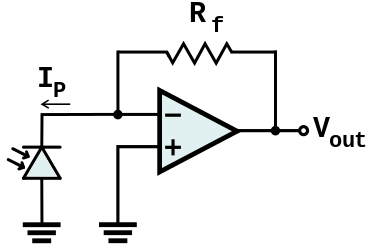
\includegraphics[width=0.8\textwidth]{fig/circuito/amp/TIA.png}
            \label{fig:circuito/amp/TIA}
        \end{figure}
        \vspace{-1em}
         \begin{figure}[H]
                %\centering
                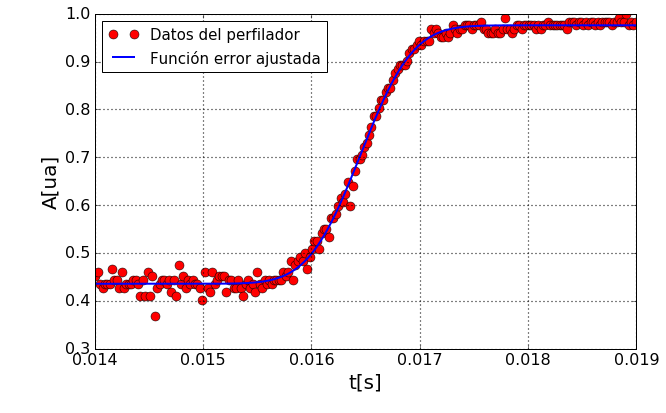
\includegraphics[width=1.2\textwidth]{fig/perfilador/fit_data_plastico_subida.png}
                \label{fig:perfilador/amplificacion_funcional}
        \end{figure}
    \end{column}
\end{columns}



\end{frame}

\begin{frame}{Calibración de amplificador}

\begin{columns}[c]
    \begin{column}{0.4\textwidth}
        \begin{itemize}
        \item Amplificador con LM358. Con fuente simple
        \item Respuesta al escalón de 0,4V$\,\mu$s$^{-1}$. 4 veces más grande de la necesaria
        \item Rango lineal bastnate amplio, pero no acusa corriente nula. Se puede buscar otro amplificador. Suficiente para la amplicación
        \end{itemize}
    \end{column}
    %
    \begin{column}{0.5\textwidth}
        \vspace{-1em}
        \begin{figure}[H]
            \centering
            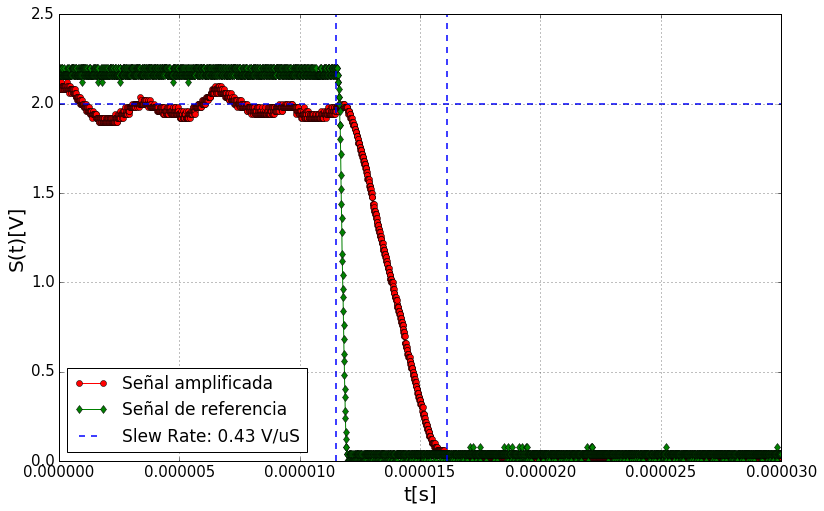
\includegraphics[width=\textwidth]{fig/circuito/amp/transicion_amp}
            \label{fig:transicion_amp}
        \end{figure}
        \vspace{-2em}
        \begin{figure}[H]
            \centering
            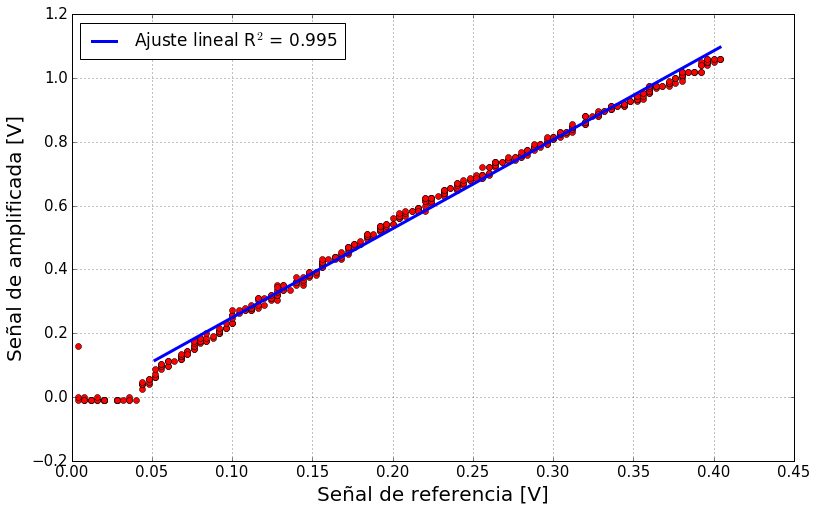
\includegraphics[width=\textwidth]{fig/circuito/amp/lin_amp}
            \label{fig:circuito/amp/lin_amp}
        \end{figure}
    \end{column}
\end{columns}


\end{frame}

\begin{frame}{Generación de sensores portátiles}
    \begin{onlyenv}<1>
        \begin{columns}[c]
            \begin{column}{.5\textwidth}
            Spark Photon
            \begin{itemize}
                \item ARM Cortex M3 120MHz con stack WiFi. 
                \item 128KiB RAM y 1MiB FLASH
                \item Programación en la nube, permite actualizaciones OTA.
                \item API de programación más poderosa. C++ por defecto
                \item Software implementado con licencia libre, puede ser adaptado
            \end{itemize}
            \end{column}

            \begin{column}{.5\textwidth}
                \vspace{-2em}
                \begin{figure}
                    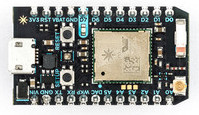
\includegraphics[width=0.8\textwidth]{fig/circuito/photon}
                    \label{fig:circuito/photon}
                \end{figure}
                
            \end{column}
        \end{columns}
    \end{onlyenv}

    \begin{onlyenv}<2>
        \begin{columns}
            \begin{column}{0.7\textwidth}
                \begin{block}{Resultados con este uC/Software}
                    \begin{itemize}
                        \item Se pudo mover el motor hasta 30RPS. \\PWM mejor implementado
                        \item Adquisición de datos (del uC) cada 10$\mu$s o 100ksps. Más de lo necesario
                        \item Conexión TCP ya resuelta, cada 0,1s se obtiene 4000 datos. 
                        \item Software de adquisición hecho enteramente en Python, libre, con interfaz de usuario gráfica
                    \end{itemize}
                \end{block}
            \end{column}
            \begin{column}{0.3\textwidth}
                \begin{figure}
                    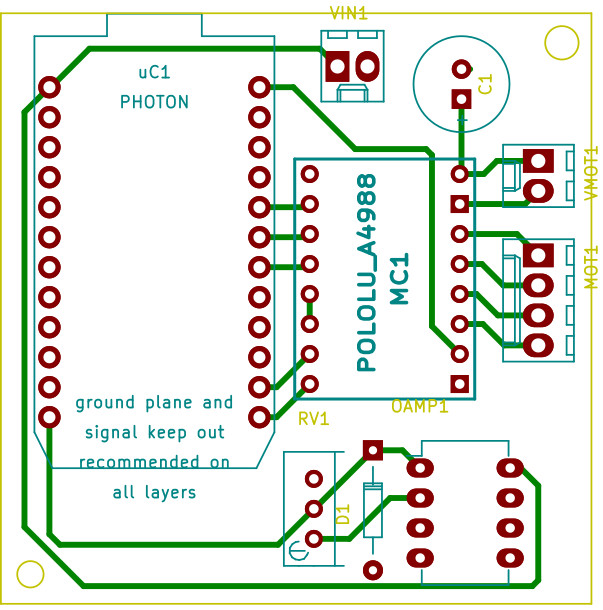
\includegraphics[width=\textwidth]{fig/circuito/circuito_labo7_color}
                    \label{fig:circuito/circuito_labo7_color}
                \end{figure}
            \end{column}
        \end{columns}
    \end{onlyenv}

\end{frame}


